% ===================================================================================
% Methodology redraft -- 2026-08-24, v3. New copy, does not overwrite 22nd_methodology_
% redraft.tex. Same overall order (Q1, Q2, Q3, Evaluation) and same equation labels as v2,
% so cross-references elsewhere keep working -- but this pass audits WORDING against the
% actual code and current results drafts (results_q1_21_08_0754pm.tex,
% results_q2_22_08_0214.tex, results_q3_23_08_0540am.tex, q2/q3 brain dumps), not just
% against the reviewer feedback v2 was built on. Evidence priority used throughout: saved
% outputs/predictions -> run configs/logs -> executed scripts -> current code -> draft ->
% working notes.
%
% Fixed this pass (verified against code, not assumed):
%   1. Q1's XGBoost description changed from "tuned parameters" to "fixed configuration,
%      adopted after a one-off comparison, not searched on this target" -- confirmed via
%      run_rq2_attribution.py:93-100 and rq1_xgb_hyperparameter_search.py's own header
%      comment ("never actually searched on RQ1's own data"). The 27-config grid search
%      that DOES exist under that filename targets elev_percentile_95th (RSQ1=Q3), not
%      Q1's mean_cr_residual -- a genuine, separate search, correctly already attributed
%      to Q3 lower down in this file.
%   2. Eval-robustness's old claim "Neural stability is checked over five seeds" had no
%      matching code anywhere -- checked run_cv_seed_sweep.py (8 seeds) and
%      run_seed_sweep_check.py (4 seeds), both reseed Elastic Net/XGBoost's SPLIT
%      assignment, not any neural network. No DNN/PINN/PINN-k multi-seed run exists in
%      this project. Rewritten to state plainly what is and is not seed-checked, and to
%      point instead at the real robustness evidence for the neural models: the
%      training-setting, physics-weight and feature-set sensitivity checks below.
%   3. PINN forward-pass module provenance disclosed explicitly: the corrected forward
%      pass (Equation~\eqref{eq:pinn-prediction}) lives only in a working-scripts copy,
%      not the shared model module -- see the new sentence after that equation.
%   4. Q3's "Row-level curve correction" subsection (old sec:rq2a-method, eq:residual-
%      reduction, CR-error-quartile check) removed: confirmed absent from the current
%      results_q3_23_08_0540am.tex (no "quartile", "d_i", or "residual-reduction"
%      anywhere in that file) -- this analysis is no longer part of the reported Q3
%      story. Replaced with a new "Sensitivity checks and diagnostics" subsection
%      describing what Q3 actually reports now (training-setting checks, physics-weight
%      ablation, feature-set sweep, terrain permutation importance, age/height error
%      banding, the compartment cross-fold check, and the yield-class correlation check).
%   5. tab:rq-framework's Q3 row updated to match (4) -- old "row-level error reduction"
%      target description and "CR-error-quartile correction" evaluation description
%      both removed.
%   6. GNNWR section gains one plain descriptive sentence: no hyperparameter search was
%      performed for it, stated as a fact about the method (not editorialised as a
%      limitation here -- the limitation framing already lives in the Limitations file).
%   7. Elastic Net's inner-loop tuning claim (Q1) confirmed accurate as written --
%      elasticnet_environmental.py:115, ElasticNetCV with an l1_ratio grid, cv=5. No
%      change needed.
%   8. GNNWR's computational-adjustments paragraph (full reference set post-GPU-cap,
%      hat-matrix diagnostics disabled, AIC uses raw feature counts) confirmed accurate
%      against gnnwr_check.py. No change needed.
%
% RE-AUDIT 2026-08-24 (second pass, full line-by-line sweep of every remaining checkable
% claim, not just the shortlist above): 18 distinct numeric/architecture claims VERIFIED
% exactly against code (60m buffer, k=5 folds, both dropped neighbour-height variables,
% separate age scaling, Spearman 0.95 dedup threshold, VIF>5 iterative, Set2's top-10,
% REML/ML switching in nlme.py, clearfell/measurement-error thresholds, 3-layer/128-unit
% trunk, PINN's lr/weight-decay/batch-size defaults, the separate 1e-5 L1 term, 16-unit
% sub-networks, XGBoost's 27-config grid, all 8 lambda values, the 512 batch-size
% alternative, 10 permutation repeats, both bootstrap counts (1000 vs 2000, confirmed not
% swapped), and all three Moran's I parameters). Two problems found and fixed:
%   - GNNWR reseed line originally said "four-survey cohort" reseeded three times -- this
%     was backwards. The actual reseed job is for the SIX-survey R^2 cell; four-survey
%     coefficient maps are single-seed. Fixed in the Evaluation and robustness paragraph.
%   - Tukey/IQR fence (eq:tukey-fences): a `models/`-only grep initially found no
%     supporting code, flagged as a possible second bad carried-over claim. Re-checked
%     properly by parsing notebook JSON source cells directly (a plain grep on the .ipynb
%     file hit a false positive inside base64-encoded image data) -- found genuinely
%     implemented in notebooks/results_q2/results_figures_q2_example_plot.ipynb, with a
%     comment explicitly citing "same rule as Q2's own target/outlier audit (Equation
%     eq:tukey-fences)". No change needed; this claim stands.
% RESOLVED: "430 plots screened" traced to documentation/plans_md/experiment_log.md
% (line ~1540) -- the broad/broad_legitimate feature set (Set4's climate+soil columns)
% drops 430 plots / 1,720 rows from real climate/soil missingness (terrain-only sets drop
% only 39 plots / 156 rows, e.g. ceh_twi's own gap, confirmed separately in
% models/common/torch_data.py:481). Produced at run time by the environmental-set loader,
% not stored in a static script -- which is why a models/-only grep couldn't find it. No
% change needed; this claim stands.
%
% Checked and left unresolved on purpose (flagged, not silently fixed):
%   - Tukey-fence/clearfell/measurement-error rule placement (Data vs Methodology) --
%     re-confirmed no evidence these are general preprocessing in
%     data_processing/clean_master_data.py. Still a placement decision, not a
%     correctness issue. % VERIFY: confirm with the user before final submission.
%   - The PINN-k parameter-separability metric (param_correlation_ymax_k) is reported for
%     the headline configuration and across the lambda ablation, but NOT yet across the
%     Set2/Set4 feature-set sweep -- a script for this was built and syntax-checked in a
%     later session but not run. % VERIFY: do not cite per-set separability numbers until
%     confirmed against outputs/run_logs/.
% ===================================================================================

%=======================================================================================
%=======================================================================================
\chapter{Methodology and Experimental Framework} \label{ch:methodology}
\section{Experimental framework}
Q1 links a plot's deviation from the baseline growth curve to environmental and management factors. Q2 tests whether place-specific relationships explain patterns that global models miss. Q3 compares models for predicting top height, and tests whether environmental inputs or Chapman--Richards guidance improve it further.

\begin{table}[!ht]
\centering
\footnotesize
\renewcommand{\arraystretch}{1.2}
\begin{tabularx}{\linewidth}{@{} l >{\raggedright\arraybackslash}X >{\raggedright\arraybackslash}X >{\raggedright\arraybackslash}X @{}}
\toprule
Q & Unit and target & Models or comparison & Main evaluation \\
\midrule
Q1 & Plot; how far a stand sits from the shared growth curve, averaged over its survey history ($\bar r_i$) -- positive means taller than expected, negative means shorter & Elastic Net, XGBoost and a linear
mixed-effects model & Spatial block CV (Elastic Net, XGBoost); LMM coefficients and variance decomposition; residual Moran's $I$ \\
Q2 & Plot; gap between a plot's own fitted height ceiling and the ceiling its yield class predicts ($\Delta y_{\max,i}$) -- positive means a higher ceiling than expected & Elastic Net, XGBoost
and GNNWR & Five-fold spatial block CV; attribution, Moran's $I$ and target audit \\
Q3 & Plot--survey row; top height itself ($H_{it}$) & CR, linear regression, random forest, XGBoost, DNN, PINN and PINN-$k$
& Five-fold spatial block CV; pooled accuracy metrics; sensitivity checks on training
settings, physics-loss weight and environmental feature-set size; permutation-importance
and age/height error diagnostics \\
\bottomrule
\end{tabularx}
\caption{\small{Units, targets and evaluation used for each question.}}
\label{tab:rq-framework}
\end{table}

\paragraph*{Data partitions and leakage control}
The four-survey cohort was the main dataset. The six-survey cohort was used as a longer-term sensitivity check. For Q1 and Q2, each plot had one summary value. For Q3, every plot-survey row was used.

Spatial-block cross-validation reduced data leakage by assigning whole forest compartments to folds, so no compartment appeared in both training and testing \cite{roberts2017Cross_C5_EVAL}. Training plots within 60\,m of validation or test plots were also removed. This reduced spatial spillover. Five folds of roughly equal size were created. In each round, three folds trained the model, one fold tuned it, and one fold tested it. Each compartment was tested once. All test predictions were then combined to calculate final performance metrics \cite{ploton2020Spatial_C5_EVAL}.


\begin{figure}[!htbp]
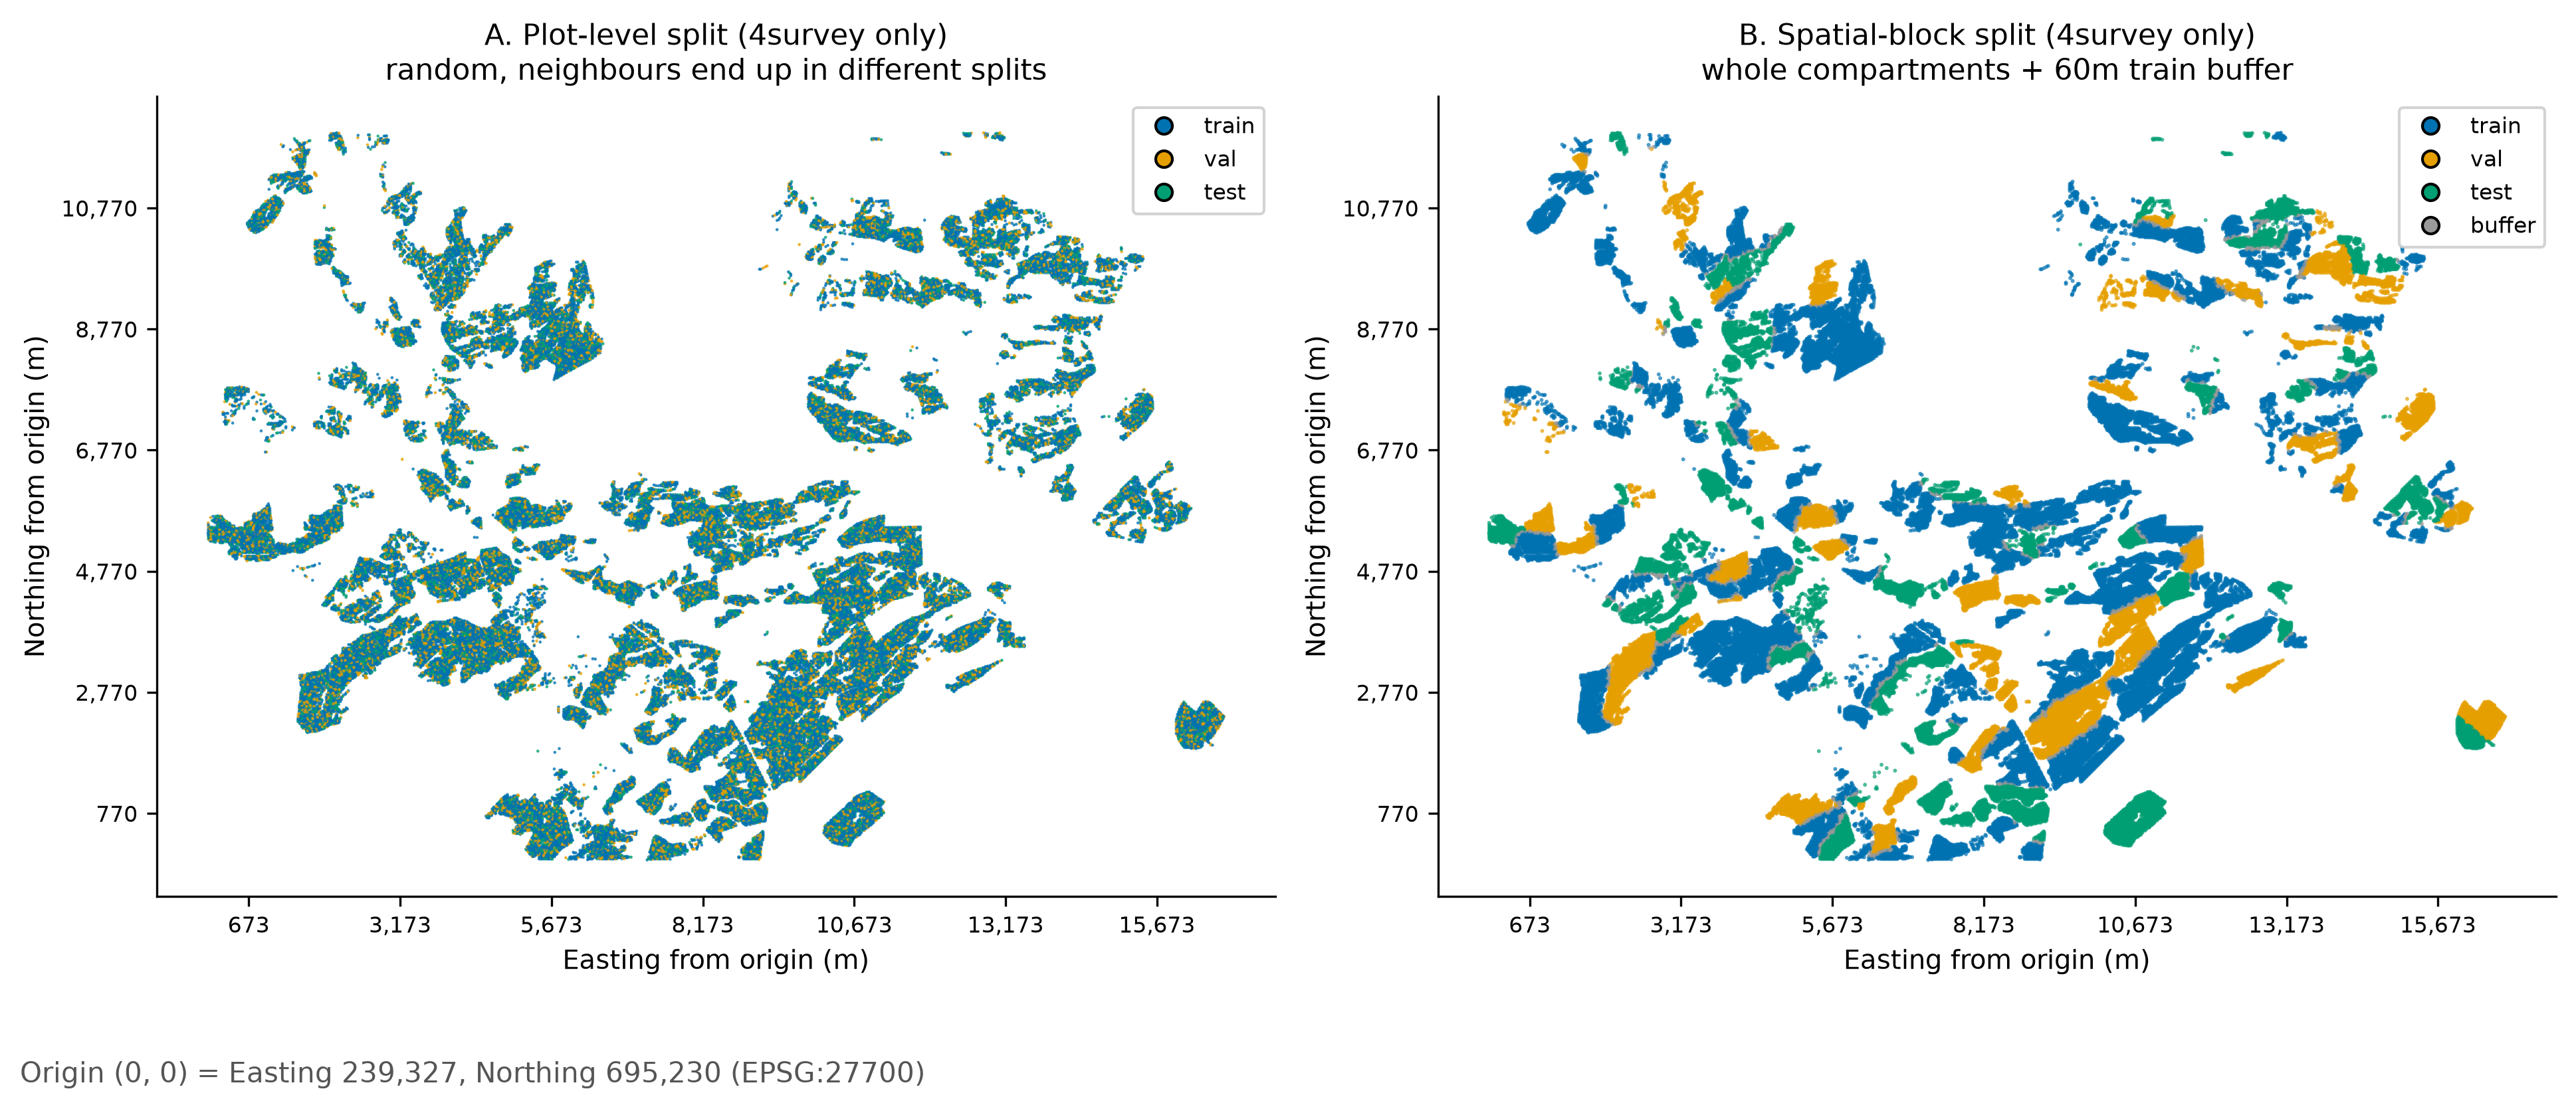
\includegraphics[width=1.0\textwidth]{figures/fig_methodology/fig_method_map_splits.png}
\centering
\caption{\small{Evaluation data-splitting strategies: (A) random plot-level split and (B) compartment-level spatial-block split with a 60\,m buffer.}}
\label{fig:splits-combined}
\end{figure} %TODO: increae font size. for axis.

Panel A: shown for context, not a reported evaluation -- an early random plot-level split inflated accuracy via leakage between neighbouring plots, motivating spatial-block CV (Panel B) instead. Random-split results are not reported in this dissertation.

Continuous variables were scaled using the training data and then applied to the validation and test sets. Age was scaled on its own so PINN outputs could be converted to metres per year. Soil types were converted to binary categories. Compartment and block IDs were left out of the models. Two neighbour-height variables were also dropped. They were built from nearby plot heights before the split, so they could leak test information.

%------------------------------------------------
\section{Environmental feature sets}
Four feature sets test whether adding more environmental information improves model performance. The sets are built separately for Q1, Q2, and Q3, so each question gets its own ranked list.

Variables with too much missing data are removed first. Exact duplicates are also removed. Near-identical variables (Spearman $|\rho|\geq0.95$) are reduced to one, and the directly measured version is kept. The remaining candidates are ranked using the mean rank across Spearman $|\rho|$, permutation importance, and drop-column ablation (both computed with XGBoost), on one spatial-block split. Variables with variance inflation factor above 5 are then removed one at a time until none remain \cite{obrien2007Caution_C5_EVAL}. Baseline variables cannot be removed, but they still count in the VIF calculation.

This screening removes 430 four-survey plots, mainly because of missing SoilGrids coverage; the six-survey cohort has no missing environmental values. Missingness details and exact membership for each question are reported in Appendix~\ref{app:feature-sets}.

\begin{table}[!htbp]
\centering
\scriptsize
\renewcommand{\arraystretch}{1.15}
\begin{tabularx}{\linewidth}{@{}p{1.4cm}X@{}}
\toprule
Set & Construction \\
\midrule

Set~1
& Stand and management baseline only. \\

Set~2
& Set~1 plus the ten highest-ranked candidates from the full environmental pool. Candidates that fail VIF screening are replaced by the next-ranked candidate. \\

Set~3
& Set~1 plus the upper-ranked half of the terrain and wind candidates, followed by VIF screening. \\

Set~4
& The Set~3 candidate categories plus the upper-ranked half of climate, soil and spatial-context candidates, followed by VIF screening across the enlarged pool. \\

\bottomrule
\end{tabularx}
\caption{Construction of the four feature sets. Ranking is target-specific, so final membership differs between Q1, Q2 and Q3. Exact lists are reported in Appendix~\ref{app:feature-sets}.}
\label{tab:feature-sets-construction}
\end{table}

The final sets are not strictly nested because VIF screening is repeated each time the candidate pool grows. For example, elevation appears in Sets~2 and~3 but is removed from Set~4 once correlated terrain and wind predictors are considered together. This shows redundancy within Set~4. It does not mean elevation is ecologically unimportant.

\section{Q1: Explaining growth deviations}
Q1 asks a simple question: once age is accounted for, which plots sit above or below the shared growth curve, and which conditions go with that difference? The analysis has two steps. First, repeated observations are reduced to one mean departure per plot. Second, Elastic Net, XGBoost, and a linear mixed-effects model explain this target. The four-survey cohort is used because the six-survey cohort has only 47 compartments, too few for reliable spatial-block comparison.

Here, $i$ marks a plot, $t$ marks a survey, $H_{it}$ and $a_{it}$ are observed height and age, and $T_i$ is the number of surveys for plot $i$. $H(a)$ is the shared Chapman-Richards growth curve (Equation~\eqref{eq:cr}) at age $a$. Equation~\eqref{eq:cr-gap} gives the gap between measured height and the baseline curve. Equation~\eqref{eq:mean-cr-residual} then averages this gap over time to give one mean departure per plot:
\begin{align}
r_{it} &= H_{it} - H(a_{it}), \label{eq:cr-gap} &
\bar{r}_i &= \frac{1}{T_i} \sum_{t=1}^{T_i} r_{it}. \label{eq:mean-cr-residual}
\end{align}
Positive $\bar{r}_i$ means observed top height is above the baseline on average. Negative means it is below. The target measures average vertical position relative to the baseline, not growth rate itself. A positive or negative mean does not mean the sign was the same at every survey. Stand age is left out of the model predictors because the growth curve already accounts for it.

Elastic Net and XGBoost are tested with five-fold spatial cross-validation. Elastic Net uses inner-loop tuning (\texttt{ElasticNetCV}, $l_1$-ratio grid, 5-fold inner CV). XGBoost uses a fixed configuration (depth 4, learning rate 0.04, up to 500 trees, early stopping). This setup was kept after a one-off comparison against defaults. It was not searched on this target. Q3's top-height XGBoost uses its own grid search instead. Pooled out-of-fold metrics ($R^2$, RMSE, MAE) give the headline estimates for both models.

To account for plots grouped within compartments, a linear mixed-effects model is fit on each fold's training partition:
\begin{equation}
\bar{r}_i = \beta_0 + \boldsymbol{\beta}^{\top}\mathbf{x}_i + u_{c[i]} + \varepsilon_i, \qquad u_c \sim \mathcal{N}(0, \sigma_u^2).
\label{eq:mixed-effects}
\end{equation}
$\boldsymbol{\beta}^{\top}\mathbf{x}_i$ is the fixed-effects term. It describes broad relationships across all plots, such as slope or TOPEX. $u_{c[i]}$ is the random intercept for plot $i$'s compartment. Each training compartment gets its own fitted intercept, drawn from a shared distribution with variance $\sigma_u^2$. This term captures unexplained grouping at compartment level. It does not identify the specific cause of that grouping. This model is used only for fitted coefficients and the variance-explained comparison below. It is not used to make held-out predictions for unseen compartments.

Parameters ($\boldsymbol{\beta}$, $\sigma_u^2$) are fitted with restricted maximum likelihood (REML). This avoids the small variance underestimate that plain maximum likelihood (ML) can give. When models with different fixed effects are compared, ML is used instead because REML likelihoods cannot be compared across different fixed-effect structures. This compares a null model (compartment random intercept only) against the full model (fixed effects added); variance explained = share of the null's compartment-level variance that shrinks once fixed effects are included. The model is refit on each fold's training data, so coefficients are reported as mean $\pm$ SD across folds. This shows fold-to-fold stability. It is different from the pooled Elastic Net and XGBoost metrics above, which measure held-out accuracy.

Two concerns motivate four checks. First, canopy cover and top height come from the same LiDAR flights. A strong canopy-cover effect could therefore reflect measurement overlap rather than real stand structure. Three steps test this: (1) refit Set~4 without canopy cover and check the change in $R^2$; (2) check the direct correlation between canopy cover and each target; (3) recompute SHAP values without canopy cover to see if other predictors take over its role.

Second, terrain coefficients for slope and TOPEX sometimes differ between Elastic Net and the mixed-effects model. This could mean local compartment effects that global models miss. A fourth check measures how much slope and TOPEX variance sits between compartments versus within them (the intraclass correlation coefficient, ICC).

Elastic Net coefficient signs, mixed-model fixed-effect signs, and XGBoost mean $|$SHAP$|$ rankings are then compared. This shows which variables matter, and in which direction when sign is available. The raw sizes are not directly comparable because the models differ, and mean $|$SHAP$|$ has no sign. Agreement across all three makes an association less likely to be a quirk of one model, but it does not show causality. Residual Moran's $I$ checks for remaining spatial clustering (Section~\ref{sec:eval-robustness}).


%------------------------------------------------
\section{Q2: Spatial attribution}
Q2 builds on Q1. Instead of asking only which variables matter overall, it asks whether their effects change by place. Global models assume one environment--growth relationship across the study area. Q2 tests whether allowing this relationship to vary by location improves explanation and reduces residual spatial clustering.

GNNWR \cite{du2020Geographically_C6_GWR} is used for this. It gives each plot a prediction that depends on its location, based on the idea that nearby plots behave more similarly than distant ones. Its coefficients can therefore vary across the map. A neural network learns these spatial weights directly from geographic coordinates, without a fixed neighbourhood size chosen in advance.

GNNWR still assumes that each local relationship is a straight line. If the real biological response is curved, a changing local coefficient may simply show that the local line fits badly there. It may not reflect a true difference in growth drivers by place. For that reason, both model accuracy and local coefficients are considered together.

\paragraph*{What Q2's target means in plain terms:} Q2 asks whether a plot's observed growth points to a higher or lower height ceiling than its assigned yield class would suggest -- does the observed trajectory imply a higher or lower fitted ceiling than its yield class predicts?

$p_1$--$p_5$ are Forest Research's published numbers that convert a yield-class rating into a full growth curve for a species and region. This project did not derive them. It only reused them. $p_1$--$p_3$ set the curve's asymptote (ceiling); $p_4$--$p_5$ set its shape (rate and curvature) -- two parts of one sigmoid. $p_4$ and $p_5$ are fixed at their published values for the matching Forest Research curve; only the height ceiling is allowed to differ from plot to plot. Earlier work has represented environmental variation through the Chapman--Richards asymptote in the same way \cite{scolforo2013Dominant_C2_CR}. This supports it as a simple and workable choice. For plot $i$ at survey $t$:
\begin{align}
g_{it} &= \left(1-e^{-p_{4,i}a_{it}}\right)^{p_{5,i}}, \label{eq:git-curve} \\
\hat y_{\max,i} &= \frac{\sum_t H_{it}g_{it}}{\sum_t g_{it}^2}, \label{eq:plot-ymax-fit} \\
y_{\max,i}^{\mathrm{yldc}} &= \mathrm{yldc}_i p_{2,i}+p_{1,i}+2p_{3,i}, \label{eq:yldc-asymptote} \\
\Delta y_{\max,i} &= \hat y_{\max,i}-y_{\max,i}^{\mathrm{yldc}}. \label{eq:local-ymax-diff}
\end{align}
With $p_4$ and $p_5$ fixed, Equation~\eqref{eq:plot-ymax-fit} gives a least-squares estimate for $\hat y_{\max,i}$. This avoids trying to estimate three correlated curve parameters from only 4--6 observations per plot. $\hat y_{\max,i}$ is the ceiling fitted from plot $i$'s own observed trajectory. $y_{\max,i}^{\mathrm{yldc}}$ (Equation~\eqref{eq:yldc-asymptote}) is the ceiling implied by its assigned yield class, using the same fixed rate and shape. Their difference, $\Delta y_{\max,i}$ (Equation~\eqref{eq:local-ymax-diff}), is positive when the fitted ceiling is higher than expected and negative when it is lower. This target is estimated, not directly observed.

Following the Q1 setup, Elastic Net and XGBoost are trained on $\Delta y_{\max}$ using Sets~2--4, with the same tuning approach as Q1. Elastic Net tests a global linear relationship. XGBoost tests a global non-linear relationship. GNNWR tests a spatially varying but locally linear relationship. Spatial variation is modelled using GNNWR via its Python library \cite{du2020Geographically_C6_GWR, du2022PyGNNWR_C6_GWR}:
\begin{equation}
\widehat{\Delta y}_{\max,i} = \beta_0(s_i) + \sum_j \beta_j(s_i) x_{ij}.
\label{eq:gnnwr}
\end{equation}
For each location $s_i$, GNNWR uses a neural network to learn spatial weights from distances to training plots. These weights determine the local coefficients $\beta_j(s_i)$ around a global linear baseline. Each training fold uses only that fold's own training partition. No hyperparameter search was performed for GNNWR. Every run uses the library's default architecture and training settings.

\subsection*{Computational adjustments and feature evaluation}
Full reference sets were used for the headline GNNWR runs. Early preliminary tests had used a smaller capped reference set because of GPU memory limits. That cap is kept only as a later sensitivity check. Memory-intensive hat-matrix diagnostics were disabled. As a result, GNNWR AIC is approximated using raw feature counts rather than the true GWR-corrected effective degrees of freedom, and $F$-tests are not reported. Predictive metrics ($R^2$, RMSE) are unaffected. Elastic Net and XGBoost were unaffected. %TODO: appendix section for full implementation detail not yet written.

Feature importance is measured with XGBoost gain, test-fold SHAP values \cite{lundberg2017Unified_C7_XAI}, and GNNWR's local coefficient distributions and maps. Each feature group's contribution to $R^2$ is measured by permutation importance, by shuffling that group's columns without refitting. Its contribution to residual clustering is measured by removing the group from Set~4 and refitting, then comparing Moran's $I$ before and after on the four-survey cohort. A separate check isolates canopy cover. Each of the three models is refit with canopy cover as the only predictor, and again with canopy cover removed, to test how much of the score depends on this one variable.

\subsection*{Target and outlier audit}
%TODO: flagged for a decision, not yet moved -- checked against data_processing/clean_master_data.py:
% no evidence found that these two rules are applied as general preprocessing elsewhere in
% this project; they appear specific to Q2's own plot-level asymptote-fitting population, which
% would make Methodology the correct home, not the Data chapter. % VERIFY: confirm before
% moving.
Plots affected by clearfelling, or by likely measurement error, are excluded from the asymptote analysis using two rules applied to consecutive surveys. (1) Clearfell: top height drops $\ge 25\%$, canopy cover drops $\ge 70\%$, and standing volume drops $\ge 70\%$. (2) Measurement error: top height drops $\ge 25\%$, while canopy cover drops $\le 10\%$ and volume does not drop. Plots with large height drops that match neither rule are kept. Extreme fitted ceilings ($\hat{y}_{\max,i}$) are identified using Tukey's $1.5\,\mathrm{IQR}$ rule \cite{tukey1977Exploratory_C5_EVAL}: % Tukey (1977) -- NB: mybibfile.bib has a near-duplicate entry (tukey1977exploratory_C5_EVAL, lowercase e) for the same book; dedupe before submission, this cites the capital-E one.
\begin{equation}
\left[Q_1 - 1.5\,\mathrm{IQR},\; Q_3 + 1.5\,\mathrm{IQR}\right].
\label{eq:tukey-fences}
\end{equation}
These bounds are computed directly from the data, not taken from a published cutoff.
Flagged plots are kept in the main runs, but tested separately by removing them from test predictions.

Top 1\% and 5\% largest-residual plots are compared for overlap across Elastic Net, XGBoost, and GNNWR, to see whether the same plots are flagged by every method. Their spatial spread, distance to stand edges, wind shelter, and local coefficients are compared against the rest of the plots, to check whether extreme errors are linked to fitting artifacts, disturbance, or environmental conditions -- a link, not a proven cause. Which plots are flagged, and what that means, is reported in Results.
% REMOVED 2026-08-24: "refit them without 2008 data" -- grepped every outlier/disturbance
% script under models/growth_curve_attribution/ (disturbance_checks.py,
% disturbance_checks_refined.py, rq3_outlier_diagnosis.py, cross_reference_outliers_with_
% disturbance.py) for "2008" and any year-exclusion refit logic; no match anywhere. Carried
% over from the old draft without ever being verified -- cut rather than left as an
% unconfirmed claim. % VERIFY: if this check was actually run under a different name/year
% variable, restore it with the correct script cited.

%------------------------------------------------
\section{Q3: Prediction and physics guidance}

Q3 compares models for predicting top height: a baseline growth curve, standard tabular models, and neural networks, including physics-informed ones. It then tests whether environmental variables or Chapman--Richards guidance improve accuracy or the interpretability of the fitted parameters. Using five spatial folds on Set~3, the other feature sets test whether adding environmental data helps.

\subsection{Chapman--Richards (CR) baseline}
\begin{equation}
H(a) = y_{\max}\left(1 - e^{-ka}\right)^p,
\label{eq:cr}
\end{equation}
where $H(a)$ is height at age $a$, $y_{\max}$ is the height ceiling, $k$ is the growth rate, and $p$ controls curve shape. All three parameters are fit freely by non-linear least squares on each training fold and then frozen, keeping test folds fully independent.

\subsection*{Conventional models}
We test three baselines: linear regression, random forest, and XGBoost \cite{chen2016XGBoost_C4_NN}. For Q3, XGBoost was tuned across 27 settings of tree count, depth, and learning rate over five folds using validation $R^2$. The winning setup was then tested on held-out data only after that choice was fixed (Appendix~\ref{app:hyperparameters}).

\subsection{DNN and physics-informed models}
All neural networks: three-layer trunk, 128 units per layer, Leaky-ReLU, Adam optimiser (learning rate $10^{-4}$, weight decay $10^{-5}$, batch size 256, early stopping) -- defaults, checked against alternatives (Sensitivity checks and diagnostics, below). Standard DNN: minimises mean squared error ($\mathcal{L}_{\mathrm{data}} = \frac{1}{N}\sum (\hat H_i-H_i)^2$). Conditioned DNN: environmental variables feed the input directly. PINN, PINN-$k$: environmental variables feed small sub-networks instead, which adjust each plot's own growth-curve parameters. Plain PINN adjusts only the height ceiling ($y_{\max}$); growth rate ($k$) and shape ($p$) stay one shared value for every plot. PINN-$k$ adjusts both $y_{\max}$ and $k$; $p$ stays shared for both variants. These per-plot parameters shape the prediction and the loss terms together -- fitting the data while staying close to the growth curve's shape.

Equations~\eqref{eq:cr-derivative}--\eqref{eq:total-loss}: the physics-informed loss.
\begin{align}
H'(a) &= y_{\max}pk e^{-ka}\left(1-e^{-ka}\right)^{p-1}, \label{eq:cr-derivative} \\
\mathcal{L}_{\mathrm{phys}} &= \frac{1}{N}\sum_{i=1}^{N}\left(\frac{\partial\hat H_i}{\partial a_i}-H'(a_i)\right)^2, \label{eq:physics-loss} \\
\mathcal{L}_{\mathrm{traj}} &= \frac{1}{M}\sum_{j=1}^{M}\left(\frac{\hat H_{j,\mathrm{later}}-\hat H_{j,\mathrm{earlier}}}{\Delta a_j}-H'(\bar a_j)\right)^2, \label{eq:trajectory-loss} \\
\mathcal{L} &= \mathcal{L}_{\mathrm{data}} + \lambda_{\mathrm{phys}}\mathcal{L}_{\mathrm{phys}} + \lambda_{\mathrm{traj}}\mathcal{L}_{\mathrm{traj}} + 10^{-5}\sum_{\theta}|\theta|. \label{eq:total-loss}
\end{align}
Equation~\eqref{eq:cr-derivative}: theoretical growth rate, shown with the shared global parameters; conditioned models substitute each plot's own adjusted parameters instead -- $y_{\max}^{(i)}$ for both PINN variants, plus $k^{(i)}$ for PINN-$k$. Equation~\eqref{eq:physics-loss}: gap between this rate and the network's own derivative ($\partial\hat H_i/\partial a_i$). Equation~\eqref{eq:trajectory-loss}: gap between consecutive-survey growth and this rate, at midpoint age $\bar a_j$. Equation~\eqref{eq:total-loss}: data loss plus weighted physics and trajectory terms, plus an L1 penalty. Defaults: $\lambda_{\mathrm{phys}}=\lambda_{\mathrm{traj}}=1$; 0 turns the physics terms off.

Sub-networks adjust plot parameters:
\begin{equation}
y_{\max}^{(i)} = y_{\max}+f_y(\mathbf{x}_i), \quad k^{(i)} = k\exp\!\left(f_k(\mathbf{x}_i)\right).
\label{eq:param-adjust}
\end{equation}
Plain PINN: $y_{\max}^{(i)}$ line only, $k^{(i)}=k$ fixed. PINN-$k$: both lines. Each sub-network in use ($f_y$ alone for PINN; $f_y$, $f_k$ for PINN-$k$): one hidden layer, 16 units, fixed by design -- turns terrain features into one number. Trunk and sub-networks train together: one Adam optimiser, one learning rate, one weight decay, no separate tuning step per part. Sub-network outputs feed the prediction directly (Equation~\eqref{eq:pinn-prediction}), so ordinary training already shapes them; $\lambda_{\mathrm{phys}}$ adds a further pull toward matching the theoretical growth rate.

The final prediction: the Chapman--Richards curve at the plot's adjusted parameters, plus a residual from the trunk:
\begin{equation}
\hat H_i = y_{\max}^{(i)}\left(1-e^{-k^{(i)}a_i}\right)^{p} + \text{trunk residual}.
\label{eq:pinn-prediction}
\end{equation}
$y_{\max}^{(i)}$ shapes the prediction directly for both variants; $k^{(i)}$ does too, for PINN-$k$. Implemented in \texttt{pinn\_env\_terrain\_fix.py} / \texttt{pinn\_env\_terrain\_k\_fix.py}.

\subsection*{Sensitivity checks and diagnostics}
Beyond five-fold spatial evaluation, six further checks test the PINN and PINN-$k$ results. Each is a single run per fold or condition, not a repeated-seed study:
\begin{itemize}
\setlength\itemsep{0pt}
\item \textbf{Training settings and physics weight.} Alternative learning-rate and weight-decay settings, an alternative batch size (512 vs.\ 256), and eight $\lambda_{\mathrm{phys}}=\lambda_{\mathrm{traj}}$ settings (0--3.0) were each tested for DNN, PINN, and PINN-$k$ over five folds, against the defaults used for every other number in this chapter.
\item \textbf{Environmental feature-set size.} PINN and PINN-$k$ were retrained with no environment, and with Sets~2, 3, and 4, over five folds each. This tests whether environmental data helps at all, and whether the exact list matters.
\item \textbf{Terrain permutation importance.} Each terrain or wind feature was shuffled in turn, with ten repeats averaged. This measures how much personalised $y_{\max}$ and $k$ change.
\item \textbf{Age- and height-banded error.} MAE was compared by age band and height band for DNN, PINN, and PINN-$k$ on the same held-out rows. This tests whether error clusters at the extremes.
\item \textbf{Exploratory compartment check.} One compartment, flagged after inspecting results for an unusually large personalised deviation, has its prediction compared across all five folds -- held out in one fold, seen in training in the other four. This separates a consistent site effect from a fold-specific generalisation failure.
\item \textbf{Yield-class comparison.} Each model's personalised parameter deviation is compared with that plot's yield class, a Forest Research site rating excluded from every model's inputs. Tested on the full test set, not only extreme cases, to check whether personalisation tracks this external site-quality measure.
\end{itemize}

\section{Evaluation and robustness} \label{sec:eval-robustness}
This final section explains how model performance and robustness are judged. Model accuracy is evaluated using RMSE, MAE, $R^2$, and Bias. Here $e_i = y_i - \hat y_i$, where $y_i$ is the relevant target: $\bar r_i$ for Q1, $\Delta y_{\max,i}$ for Q2, and top height for Q3.
\begin{equation}
\mathrm{RMSE}=\sqrt{\tfrac{1}{N}\textstyle\sum e_i^2}, \quad
\mathrm{MAE}=\tfrac{1}{N}\textstyle\sum |e_i|, \quad
R^2=1-\tfrac{\sum e_i^2}{\sum (y_i-\bar y)^2}, \quad
\mathrm{Bias}=\tfrac{1}{N}\textstyle\sum e_i.
\label{eq:eval-summary}
\end{equation}
Positive bias indicates under-prediction. We report fold-level means ($\pm\text{SD}$) or pooled metrics across all out-of-fold predictions. For the 4-survey cohort, $R^2$ $95\%$ confidence intervals are calculated using 1,000 compartment bootstrap resamples.

Residual spatial autocorrelation is measured using global Moran's $I$:
\begin{equation}
I=\frac{N}{W}\frac{\sum_i\sum_j w_{ij}(e_i-\bar e)(e_j-\bar e)}{\sum_i(e_i-\bar e)^2}.
\label{eq:morans-i}
\end{equation}
Spatial weights ($w_{ij}$) use binary, row-standardised distance bands matched to each model's own semivariogram range (up to 5,000\,m; 999 permutations). When needed, rows are subsampled to 5,000 to keep this fast to compute. Moran's $I$ is left out if semivariance is flat. It is marked provisional if semivariance keeps rising past 5,000\,m. Distances are reported alongside every value. Because each model's band is fitted to its own residual surface, Moran's $I$ values are comparable in direction across models, but not as exact like-for-like magnitudes.

\limit{Global Moran's $I$ detects spatial structure without identifying its cause, and equal-and-opposite local clusters may go undetected. A lower Moran's $I$ reflects less clustering, not lower overall error variance.}

Seed-based stability: checked only where actually run, not uniform across models. Elastic Net, XGBoost: split assignment reseeded over eight seeds, both cohorts -- tests sensitivity to the spatial partition, not to model training. For GNNWR, the 6-survey $R^2$ cell was re-run across three different splits, since GNNWR has no separate training seed to change; the 4-survey local maps were left on a single run. DNN, PINN, PINN-$k$: one seed per fold, no split- or training-seed repetition -- robustness for these three instead comes from the training-setting, physics-weight, and feature-set checks above.

For PINN-$k$, parameter separability is measured by the correlation between predicted $y_{\max}$ and $k$ using 2,000 compartment bootstrap resamples. This is reported alongside $R^2$ for the headline configuration and across the physics-weight ablation, because improving this separation is one aim of the physics loss. %TODO: the same separability metric across the Set2/Set4 feature-set sweep was built and syntax-checked in a later session but not yet run/verified -- do not cite specific per-set separability numbers until confirmed against outputs/run_logs/, matching this project's own verification convention.
